\documentclass{article}

%\usepackage[T1]{fontenc}
%\usepackage[utf8]{inputenc}
%\usepackage{polski}
\usepackage[utf8]{inputenc}
\usepackage{polski}
\usepackage[polish]{babel}
\usepackage{mathtools}
\usepackage[thinc]{esdiff}
\usepackage{graphicx} 

\usepackage{float}

\usepackage{geometry}

\begin{document}
\newgeometry{tmargin =3cm, bmargin=3cm, lmargin=3cm, rmargin=3cm}
\begin{tabular}{|c|c|c|}
\hline 
\multicolumn{3}{|c|}{\huge Sprawozdanie } \\ 
\hline 
\multicolumn{3}{|c|}{\LARGE Projekt 1  NMTS} \\ 
\hline 
\Large Przygotowali: &\Large Piotr Pietruszka 171842 &\Large Marcin Wankiewicz 172118  \\ 
\hline 
\Large Kierunek: ACiR  \\ 
\hline 
 
\end{tabular} 

\section{Modele stanowe bez kontrolera}

\subsection{Model ciągłoczasowy}

\begin{equation}\label{eq:q_y}
 \begin{array}{l}
  q = \alpha_1 \rho_f g (H_1 - H_2) \\
  y = \alpha_2 \rho_f g H_2
\end{array}
\end{equation}

Równania dynamiki dla zadanego systemu  \ref{eq:H_1_2}.
\begin{equation}\label{eq:H_1_2}
 \begin{array}{l}
  \diff{H_1}{t} = \frac{u-q}{S_1} \\
  \diff{H_2}{t} = \frac{q-y}{S_2}
 \end{array}
\end{equation}

Z równań \ref{eq:H_1_2} oraz \ref{eq:q_y}, przyjmując $H_1$ i $H_2$ jako zmienne stanu, uzyskano ciągłoczasowy model stanowy \ref{eq:ss_cont}.
\begin{equation}\label{eq:ss_cont}
 \begin{array}{l}
 
 \begin{bmatrix} \dot{H_1} \\ \dot{H_2} \end{bmatrix}  = 
 \begin{bmatrix} -\frac{\alpha_1 \rho_f g}{S_1} & \frac{\alpha_1 \rho_f g}{S_1}\\ 
  \frac{\alpha_1 \rho_f g}{S_2} & -\frac{\alpha_1 \rho_f g + \alpha_2 \rho_f g}{S_2} 
 \end{bmatrix}   \begin{bmatrix} H_1 \\ H_2 \end{bmatrix} + 
 \begin{bmatrix}\frac{1}{S_1} \\ 0\end{bmatrix}u  \\
 
 y[n]  = \begin{bmatrix} 0 & \alpha_1 \rho_f g \end{bmatrix}
 \begin{bmatrix} H_1 \\ H_2 \end{bmatrix} + 
 \begin{bmatrix} 0 \end{bmatrix} u[n]
 
 \end{array}
\end{equation}

Po podstawieniu wartości liczbowych, zgodnie ze standardowymi oznaczeniami macierzy uzyskano ciągłoczasowy model w przestrzeni stanu: \ref{eq:ss_cont_val}.

\begin{equation}\label{eq:ss_cont_val}
 \begin{array}{l}
  \mathbf{A} = \begin{bmatrix}  -0.00111111 &  0.00111111 \\
  							    0.004      & -0.008    
  			   \end{bmatrix} \\ \\
  \mathbf{B} = \begin{bmatrix} 0.11111111 \\ 0 \end{bmatrix} \\ \\
  \mathbf{C} = \begin{bmatrix} 0 & 0.01 \end{bmatrix} \\ \\
  \mathbf{D} = \begin{bmatrix} 0 \end{bmatrix} \\
\end{array}
\end{equation}

Transmitancję układu w dziedzinie $s$ przedstawiono w równaniu: \ref{eq:cont_transf}.
\begin{equation}\label{eq:cont_transf}
 \begin{array}{l}
  \frac{4.44444444 \cdot 10^{-6}}{ s^2 + 9.11111111\cdot 10^{-3}s + 4.44444444 \cdot 10^{-6}}
\end{array}
\end{equation}

Model nie ma zer i posiada 2 bieguny rzeczywiste, ujemne: $-0.00859395$ i $-0.0005171$. Graficznie przedstawiono je na rys. \ref{fig:cont_poles}. Brak urojonych części biegunów oznacza, że odpowiedź skokowa układu (rys. \ref{fig:step_resp_cont}) nie posiada oscylacji. 

\begin{figure}[H]
    \centering
    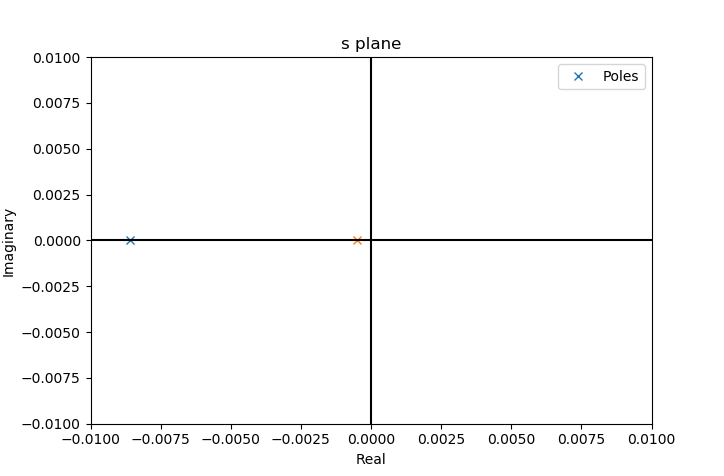
\includegraphics[width=0.7\textwidth]{img/cont_poles.png}
    \caption{Bieguny układu, model ciągłoczasowy}
    \label{fig:cont_poles}
\end{figure}

\begin{figure}[H]
    \centering
    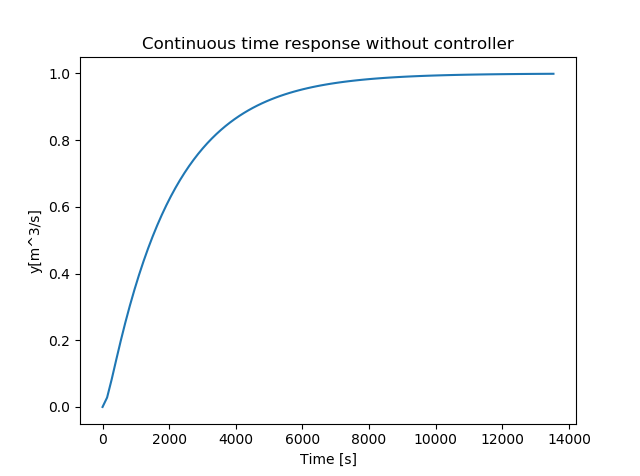
\includegraphics[width=0.7\textwidth]{img/step_resp_cont.png}
    \caption{Odpowiedź skokowa, model ciągłoczasowy}
    \label{fig:step_resp_cont}
\end{figure}

\subsection{Model dyskretnoczasowy}
Następnie model ciągłoczasowy przekształcono do dyskretnoczasowego modelu w przestrzeni stanu \ref{eq:ss_disc_val}, przy użyciu funkcji $cont2discrete$, z biblioteki $scipy.signal$. Użyto domyślnej metody dyskretyzacji (ang. zero-order hold). Przyjęto czas próbkowania równy $401.05s$, czyli $\frac{1}{15}$ czasu, w którym odpowiedź skokowa osiąga wartość 0.95.
\begin{equation}\label{eq:ss_disc_val}
 \begin{array}{l}
  \mathbf{A_d} = \begin{bmatrix}  0.75526739 & 0.10741822 \\
  							     0.3867056  & 0.08927442 
  			   \end{bmatrix} \\ \\
  \mathbf{B_d} = \begin{bmatrix} 38.2046993 \\ 13.73143858 \end{bmatrix} \\ \\
  \mathbf{C_d} = \begin{bmatrix} 0 & 0.01 \end{bmatrix} \\ \\
  \mathbf{D_d} = \begin{bmatrix} 0 \end{bmatrix} \\
\end{array}
\end{equation}

Transmitancję układu w dziedzinie $z$ przedstawiono w równaniu: \ref{eq:disc_transf}.
\begin{equation}\label{eq:disc_transf}
 \begin{array}{l}
  \frac{0.13731439 z + 0.04403063}{ z^2 - 0.84454181 z + 0.02588683}
\end{array}
\end{equation}

Model dyskretnoczasowy posiada 2 bieguny: $0.81268849$ i $0.03185333$ oraz jedno zero: $-0.32065564$. Graficznie przedstawiono je na rys. \ref{fig:disc_poles}. Odpowiedź skokową układu zamieszczono na rys. \ref{fig:disc_poles}.

\begin{figure}[H]
    \centering
    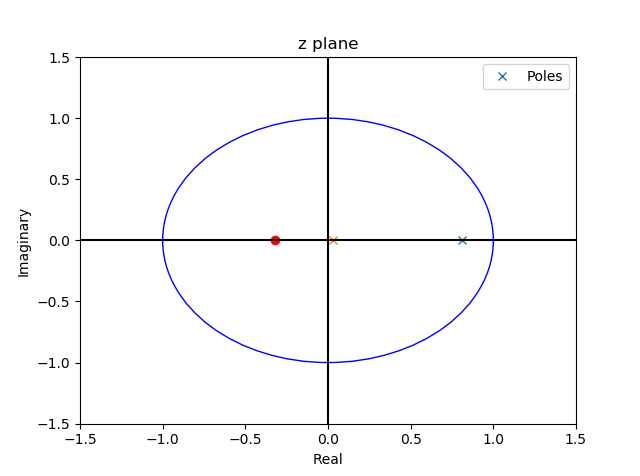
\includegraphics[width=0.7\textwidth]{img/disc_poles.png}
    \caption{Bieguny układu, model dyskretnoczasowy}
    \label{fig:disc_poles}
\end{figure}

\begin{figure}[H]
    \centering
    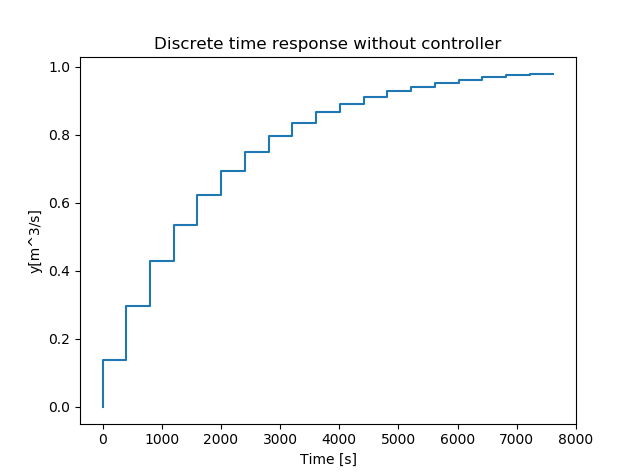
\includegraphics[width=0.7\textwidth]{img/step_resp_disc.png}
    \caption{Odpowiedź skokowa, model dyskretnoczasowy}
    \label{fig:step_resp_disc}
\end{figure}




\begin{equation}\label{eq:stan_disc}
 \begin{array}{l}
  \mathbf{x}[n+1] = \mathbf{A}\mathbf{x}[n] + \mathbf{B}\mathbf{u}[n] \\
  \mathbf{y}[n]= \mathbf{C} \mathbf{x}[n] + \mathbf{D}\mathbf{u}[n]
\end{array}
\end{equation}














\section{Templates - do usuniecia}
\begin{equation}\label{eq:standard_ss_template}
 \begin{array}{l}
  \mathbf{A} = \begin{bmatrix}  1 & 1 \\
  							   1 & 1 
  			   \end{bmatrix} \\ \\
  \mathbf{B} = \begin{bmatrix} 1 \\ 1 \end{bmatrix} \\ \\
  \mathbf{C} = \begin{bmatrix} 1 & 1 \end{bmatrix} \\ \\
  \mathbf{D} = \begin{bmatrix} 0 \end{bmatrix} \\
\end{array}
\end{equation}



\end{document}


